%%% BEGIN CHAPTER 4 MICROARRAY %%%

%% Paper title page %%
\chapter{Folding and misfolding of potassium channel monomers during assembly and tetramerization}
\section{Introduction}

In Chapter 3, we developed a KcsA monomer mutant that retains its native-like structure more than the wild-type (WT) does by engineering a disulfide bridge near the ends of the 2 transmembrane (TM) helices. Here in this chapter, we compare the folding kinetics of WT and the disulfide-bridged (CC) KcsA mutant with and without the C-terminal "tetramerization" domain. The refolding studies reveal several interesting aspects about potassium channel folding. First, the WT KcsA folding displays a biphasic kientic behavior with fast and slow processes with $\tau_{f} \sim$ 50 and 1400 seconds, respectively. However, in the CC mutant, only the fast process is present, suggesting that locking the 2 TM helices with a disulfide bond minimizes its proclivity to misfold. Secondly, WT and CC without the C-terminal "tetramerization" domain does not have any concentration dependence despite the fact that the native state is a tetramer. Thirdly, WT and CC with the C-terminal "tetramerization" domain does fold with concentration dependence in the range of 1 - 10 $\mu$M concentration. Lastly, through ensemble FRET measurements, we propose that KcsA monomers form a dense protein-rich phase in the membrane first and fold into native structures from this phase.

\section{Methods}
\subsection{Refolding KcsA protocol}

Refolding experiments were adapted from Komarov et al.17 Briefly, desired amounts of soyPC lipids (Avanti) was dried under nitrogen gas to form a thin film and further dried under vacuum overnight. Dried lipid mixture was brought up to 10 mg/mL concentration by rehydrating the thin lipid film with Buffer B (50 mM NaPi, 100 mM NaCl, pH 6.5). This mixture was rotated for 30 minutes at room temperature, and then, in order to form small unilameller vesicles, the mixture was sonicated using a bath sonicator for 15 minutes at room temperature.

\begin{figure}[!ht]
\begin{center}
	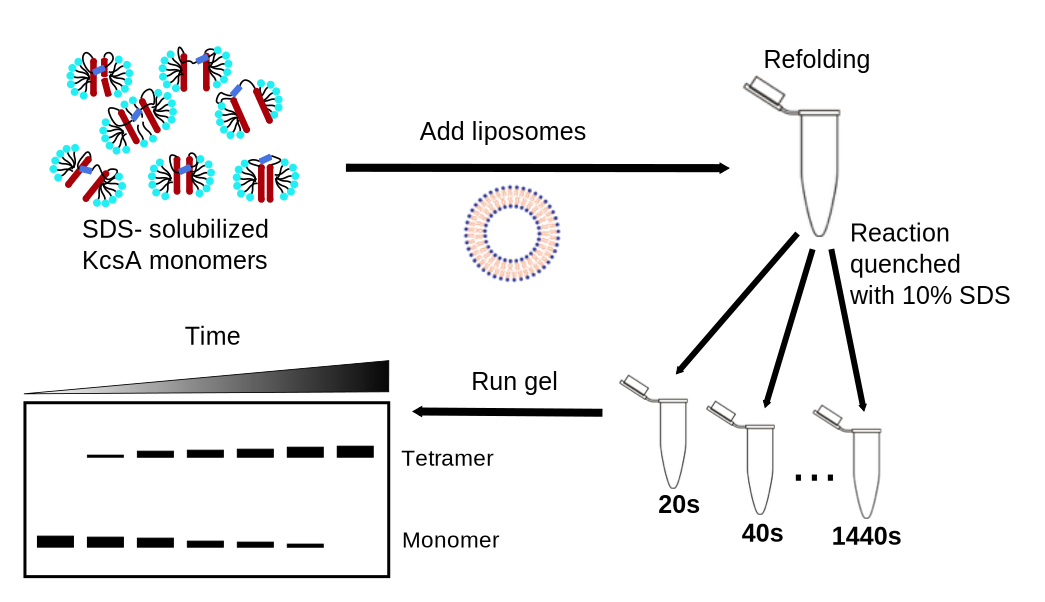
\includegraphics[width=\textwidth]{figures/chapter4/Fig4-1_refolding_protocol.pdf}
\end{center}
	\caption{\textbf{Structure of KcsA (PDB ID: 1R3J) shown from different angles}. \textbf{(A)} KcsA shown from the extracellular side of the membrane. \textbf{(B)} KcsA shown from the side. \textbf{(C)} KcsA viewed from the side with 2 monomers removed for better visualization of the selectivity filter. The oxygen atoms lining the selectivity region is rendered in Licoriche mode and the protein structures are rendered in New Cartoon mode in VMD. Each monomer of KcsA is colored in grey, blue, orange and red.}
	\label{fig:ch4_f1}
\end{figure}

Prior to refolding, precipitated KcsA $\Delta$125 monomers were solubilized in 0.5\% SDS in Buffer B with roughly protein concentrations of ~1.8 mg/mL. To initiate refolding, the protein mixture was diluted 10-fold into the refolding buffer containing asolectin vesicles. Then, at each time point a small aliquot of the refolding mixture was taken out and the reaction was quenched by diluting into 10\% SDS in Buffer B at 1:2 ratio. These quenched reaction mixtures were then run on a Novex Tris-glycine 4 – 20\% SDS-PAGE gel (ThermoFisher).

\subsection{Kinetics analysis}
	For analysis, gel images were taken with a Bio-rad ChemiDoc instrument. Then, the image was processed using ImageLab software to enhance the contrast between the protein bands and the background. For quantifying tetramer to monomer ratio, ImageJ software’s gel analysis tool was used. Each lane was normalized to itself by calculating the $\frac{[Tetramer]}{[Tetramer]+[Monomer]}$ ratio. For fitting, a double exponential function in the form of
	\begin{equation} a-be^{-\frac{t}{c}}-de^{-\frac{t}{e}} \end{equation}
was used and fitted using Scipy.optimize package in python.

\subsection{F\"{o}rster resonance energy transfer (FRET) of KcsA in liposomes}
For the site of dye conjugation, L86 in KcsA was chosen. The L86C mutation was obtained using the QuickChange protocol. Protein was expressed and purified as discussed above. Conjugation of either Cy3 or Cy5 maleimide (Kerafast) was done by overnight incubation at 4 $^{\circ}$C. Excess dye molecules were removed by size-exclusion chromatography using Superdex 200 Increase column (\textbf{Fig. \ref{fig:ch4_f2}} 

\begin{figure}[!ht]
\begin{center}
	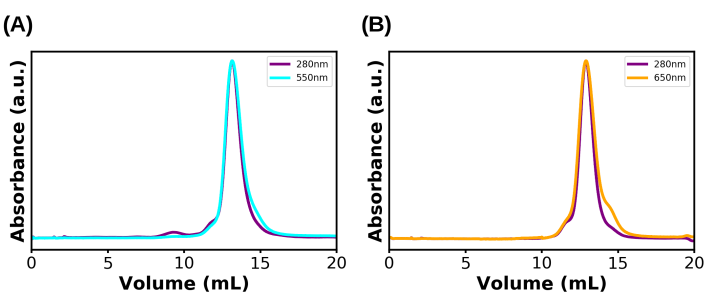
\includegraphics[width=\textwidth]{figures/chapter4/sec_cy3_cy5.pdf}
\end{center}
	\caption{\textbf{Structure of KcsA (PDB ID: 1R3J) shown from different angles}. \textbf{(A)} KcsA shown from the extracellular side of the membrane. \textbf{(B)} KcsA shown from the side. \textbf{(C)} KcsA viewed from the side with 2 monomers removed for better visualization of the selectivity filter. The oxygen atoms lining the selectivity region is rendered in Licoriche mode and the protein structures are rendered in New Cartoon mode in VMD. Each monomer of KcsA is colored in grey, blue, orange and red.}
	\label{fig:ch4_f2}
\end{figure}


Conjugation efficiency was calculated by the following equation:



\begin{equation}
	\mathrm{Conjugation\ Efficiency} = \frac{\epsilon_{dye}\alpha_{dye}}{\epsilon_{prot}\alpha_{280nm}+\epsilon_{dye}\alpha_{dye}}
\end{equation}

where $\epsilon_{prot}$ for KcsA is 33,460 cm$^{-1}$ M$^{-1}$, $\epsilon_{dye}$ = 150,000 cm$^{-1}$ M$^{-1}$ for Cy3 and 250,000 cm$^{-1}$ M$^{-1}$ Cy5, respectively, and absorbances ($\alpha_{280nm}$, $\alpha_{dye}$) were measured at 280 nm for KcsA, 550 nm for Cy3 and 650 nm for Cy5. The conjugation efficiency for both Cy3 and Cy5 samples were calculated to be ~50\%. FRET measurements were conducted with a Horiba Fluorolog-3 machine with Synapse OE-CCD Array Detector with an excitation wavelength $\lambda_{Ex}$= 500 nm. All samples contained 10 mg/mL SoyPC lipids with varying concentrations of proteins up to 10 $\mu$M.

\section{Results and Discussion}

\subsection{Kinetics of folding}

The kinetics of tetramerization of KcsA $\Delta$125 channels were examined by tracking the formation of native tetramers using an SDS resistance assay.31 The refolding protocol started with tricholoroacetic acid (TCA)-precipitated monomers solubilized with 14 mM (~0.5\% w/v) SDS at pH 6.5 (\textbf{Fig. \ref{fig:ch4_f1}A}). To initiate tetramerization, these monomers were diluted 10-fold into refolding buffer containing 14 mM asolectin liposomes. Control experiments employing dynamic light scattering verified that the liposomes remain intact after mixing with the SDS solubilized

KcsA $\Delta$125 or the 14 mM SDS buffer (Table. \ref{table:ch4_t1}). To measure refolding, aliquots of the protein-liposome mixture were removed over 25 minutes and quenched in 220 mM (~6\%) SDS buffer to arrest tetramer formation. At this high SDS concentration, liposomes were disrupted and only native tetramers persisted whereas weakly associated species were broken up and ran as monomers on SDS-PAGE gels.15-16, 31-32 The folding kinetics were quantified from the change in the gel band intensities.

\begin{table}[h]
\centering
	\caption{Folding monitored by SDS-Page gel.}
	\begin{tabular}{ccccc}
	\hline
           & WT $\Delta$125     & CC $\Delta$125      & WT FL     & CC FL                  \\
	\hline                                                                 
	\begin{tabular}[c]{@{}c@{}}Fast time\\ constant (s)\end{tabular} & \multicolumn{2}{c}{40 $\pm$ 2}     & \multicolumn{2}{c}{90 $\pm$ 10}     \\
Fast population    & \begin{tabular}[c]{@{}c@{}}0.25 $\pm$ 0.05 \\ (0.33 $\pm$ 0.05\\ 0.36 $\pm$ 0.05\\ 0.20 $\pm$ 0.05)\end{tabular} & \begin{tabular}[c]{@{}c@{}}0.86 $\pm$ 0.05\\ (0.86 $\pm$ 0.05\\ 0.83 $\pm$ 0.05\\ 0.87 $\pm$ 0.05)\end{tabular} & \begin{tabular}[c]{@{}c@{}}0.42 $\pm$ 0.04\\ (0.38 $\pm$ 0.04\\ 0.26 $\pm$ 0.04\\ 0 $\pm$ 0.04)\end{tabular} & \begin{tabular}[c]{@{}c@{}}0.55 $\pm$ 0.04\\ (0.44 $\pm$ 0.04\\ 0.16 $\pm$ 0.04\\ 0.13 $\pm$ 0.04)\end{tabular} \\
	\begin{tabular}[c]{@{}c@{}}Slow time\\ constant (s)\end{tabular} & \multicolumn{2}{c}{1500 $\pm$ 100} & \multicolumn{2}{c}{8400 $\pm$ 1600} \\
Slow population    & \begin{tabular}[c]{@{}c@{}}0.77 $\pm$ 0.03 \\ (0.70 $\pm$ 0.03\\ 0.68 $\pm$ 0.03\\ 0.83 $\pm$ 0.03)\end{tabular} & \begin{tabular}[c]{@{}c@{}}0.09 $\pm$ 0.03\\ (0.14 $\pm$ 0.03\\ 0.14 $\pm$ 0.03\\ 0.26 $\pm$ 0.03)\end{tabular} & \begin{tabular}[c]{@{}c@{}}0.59 $\pm$ 0.02\\ (0.63 $\pm$ 0.02\\ 0.76 $\pm$ 0.02\\ 1 $\pm$ 0.02)\end{tabular} & \begin{tabular}[c]{@{}c@{}}0.40 $\pm$ 0.02\\ (0.57 $\pm$ 0.02\\ 0.83 $\pm$ 0.02\\ 0.88 $\pm$ 0.02)\end{tabular} \\	\hline                
	\end{tabular}
	\label{table:ch4_t1}
	\end{table}
	
For KcsA $\Delta$125 monomers at 10 $\mu$M monomer concentration, two nearly equal refolding populations were observed, one that folded on sub-minute and another that folded on the 10 minute time scale (\textbf{Fig. \ref{fig:ch4_f3}}). Since the buildup of native tetramers is directly measured, the fast and slow appearance of native tetramers implies that there are multiple routes to the native state, rather than each phase representing a step on a sequential pathway, which would have resulted in a 10 minute lag in the buildup of tetramers.

\begin{figure}[!ht]
\begin{center}
	\includegraphics[width=\textwidth]{figures/chapter4/Fig4-2_kinetics.pdf}
\end{center}
	\caption{\textbf{Proposed KcsA folding and tetramerization.} SDS-solubilized monomers enter the liposomes and undergo rapid association into a protein-rich phase within the membrane prior to tetramerization. Oligomers can form with a native or non-native TM helical arrangement, which fold on the minute or 20 minute time scale, respectively, The rate limiting step on the faster pathway is proposed to involve the insertion of the pore helix to stabilize the tetramer in its native conformation.}
	\label{fig:ch4_f3}
\end{figure}

For the disulfide bonded CC construct, essentially all the monomers tetramerized at the fast rate (\textbf{Fig. \ref{fig:ch4_f3}}). This difference implied that the presence of unconstrained TM helices enabled the formation of a stably misfolded, slow folding species. Data for the WT and CC were fit globally, assuming the rates of the two phases were the same for the two versions. The resulting time constants were $\tau_{fast}$ = 40 $\pm$ 2 s and $\tau_{slow}$ = 1500 $\pm$ 100 s, with a 28 $\pm$ 6\% and 74 $\pm$ 6\% fast folding population for the WT and CC constructs, respectively.

\begin{figure}[!ht]
\begin{center}
	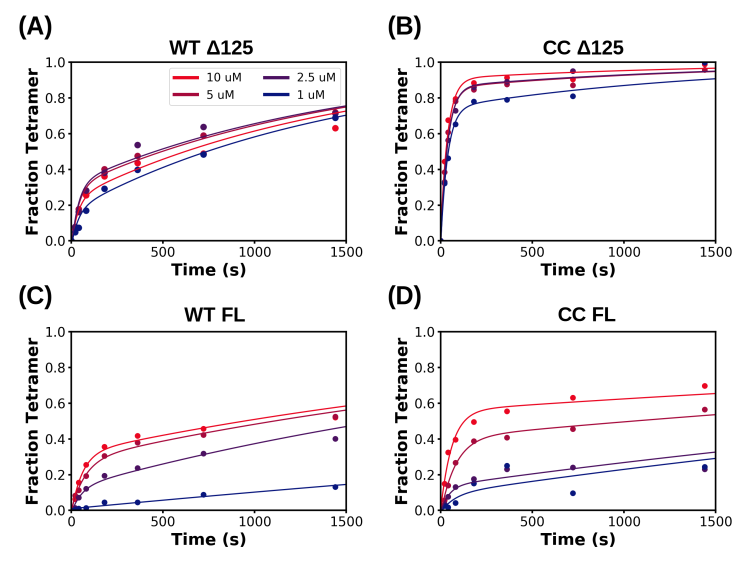
\includegraphics[width=\textwidth]{figures/chapter4/Fig4-3_conc_dependence.pdf}
\end{center}
	\caption{\textbf{Proposed KcsA folding and tetramerization.} SDS-solubilized monomers enter the liposomes and undergo rapid association into a protein-rich phase within the membrane prior to tetramerization. Oligomers can form with a native or non-native TM helical arrangement, which fold on the minute or 20 minute time scale, respectively, The rate limiting step on the faster pathway is proposed to involve the insertion of the pore helix to stabilize the tetramer in its native conformation.}
	\label{fig:ch4_f4}
\end{figure}

Next, the concentration dependence of the folding rates was studied. Interestingly, the tetramerization process, both in rate and branching ratio, appeared to be concentration independent from 1 to 10 $\mu$M within the accuracy of our measurements (\textbf{Fig. \ref{fig:ch4_f4}, Table. \ref{table:ch4_t1}}). This striking result indicates that the rate-limiting step in the folding process is a unimolecular process, despite the native state being a tetramer. If tetramerization was limited by the association of four monomers or two unstable dimers, one would have observed a 1000-fold slowing for a 10-fold decrease in concentration. As no measurable slowing was found, we propose that the oligomerization process occurs early and is fast on both routes, with the rate-limiting step representing a productive folding (fast pathway) or error-correction step (slow pathway). This proposal and the nature of this fast oligomerization process are investigated further with FRET below.

\subsection{FRET measurements suggest a formation of protein-rich phase}
The SDS folding assay indicated that the folding of both the WT and CC constructs has a minimal concentration dependence implying that the rate-limiting step is a unimolecular process. This step seems likely to occur after oligomerization in the liposomes. In principle, however, the insertion of monomers into the liposomes could be rate limiting. To test whether oligomerization is fast and occurs before the rate-limiting step, ensemble FRET measurements were carried out.

\begin{figure}[!ht]
\begin{center}
	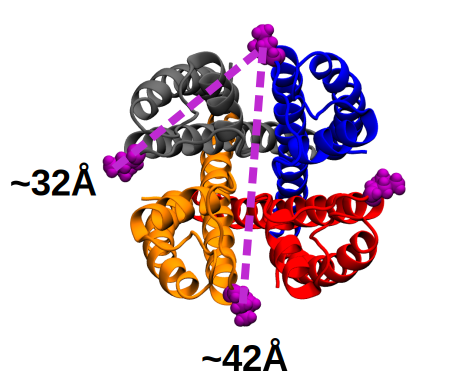
\includegraphics[width=8cm]{figures/chapter4/Fig4-4_fretpos.pdf}
\end{center}
	\caption{\textbf{Structure of KcsA with position L86C in purple.} Cy3 and Cy5 dyes were conjugated to position L86C, and mixed at a 1:1 ratio which results in two potential FRET distances of 32 and 42 Å.}
	\label{fig:ch4_f5}
\end{figure}

Dyes were first attached using thiol-labeling at a single position using a KcsA $\Delta$125 L86C variant (\textbf{Fig. \ref{fig:ch4_f5}}). Equal mixtures of donor (Cy3) and acceptor (Cy5) labeled KcsA $\Delta$125 were mixed and diluted 10-fold into the liposome mixture to initiate folding and the transfer of fluorescence was monitored (\textbf{Fig. \ref{fig:ch4_f6}}). Initially, the emission spectrum was dominated by that of the donor implying that most molecules began as isolated monomers. Upon dilution into a liposome mixture, the donor emission maximum at 570 nm was quenched by 71\% within the 10 second manual mixing dead-time while the acceptor’s emission at 680 nm increased by 7.6-fold. During the next 25 minutes over which tetramer formation occurred, only a 4\% increase in intensity was observed across the entire emission spectrum. 

\begin{figure}[!ht]
\begin{center}
	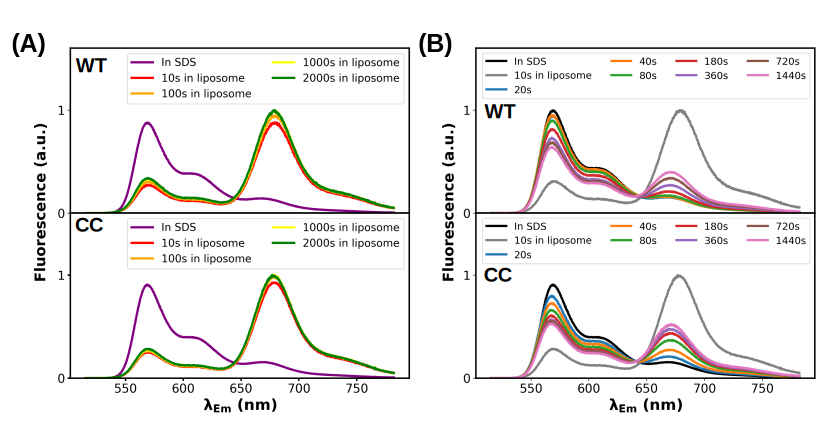
\includegraphics[width=\textwidth]{figures/chapter4/Fig4-5_fretdata.pdf}
\end{center}
	\caption{\textbf{FRET measurements of KcsA tetramerization.} \textbf{(A)} Ensemble FRET measurement of the KcsA monomer in SDS and in liposome as a function of time \textbf{(B)} Double-jump (unfold-fold-unfold) FRET measurements of KcsA refolding quenched with 10\% SDS overlaid with ‘in sds’ and ‘10s in liposome time points’ from \textbf{(A)}. Spectra are normalized to have the same value at 641 nm, an empirical iso-emissive point. Measurements are conducted at a monomer concentration of 10 $\mu$M.}
	\label{fig:ch4_f6}
\end{figure}

This biphasic FRET signal is interpreted as follows. The initial FRET increase indicates that the monomers labeled with donor and acceptor dyes rapidly associate in the liposomes prior to tetramerization. The minimal subsequent change implies that the FRET level in the rapidly associated monomers is similar to the level of folded tetramers in liposomes. The observation that most of the change in FRET signal occurred before significant tetramer formation, along with an estimate of $\sim$ 30 –- 300 monomers per liposome at 1 –- 10 $\mu$M monomer concentration, argues that most of the population forms a non-native oligomeric state upon insertion into liposomes with a FRET level comparable to that of native tetramers. The oligomers may become part of a protein-rich phase within the membrane.

To examine the possibility that FRET occurred within protein aggregates forming outside of liposomes, SDS-solubilized KcsA monomers were diluted 10-fold into water in the absence of liposomes. In this control, the overall donor fluorescence decreased 4\%, but the acceptor fluorescence spectrum only had a minimal indication of FRET (Fig. \ref), especially as compared to refolding in liposomes. The signal decrease indicates that some fraction of monomers was no longer in solution; however, more importantly, the lack of significant FRET indicates that the large observed FRET changes in the presence of liposome only came from membrane-solubilized proteins.

\begin{figure}[!ht]
\begin{center}
	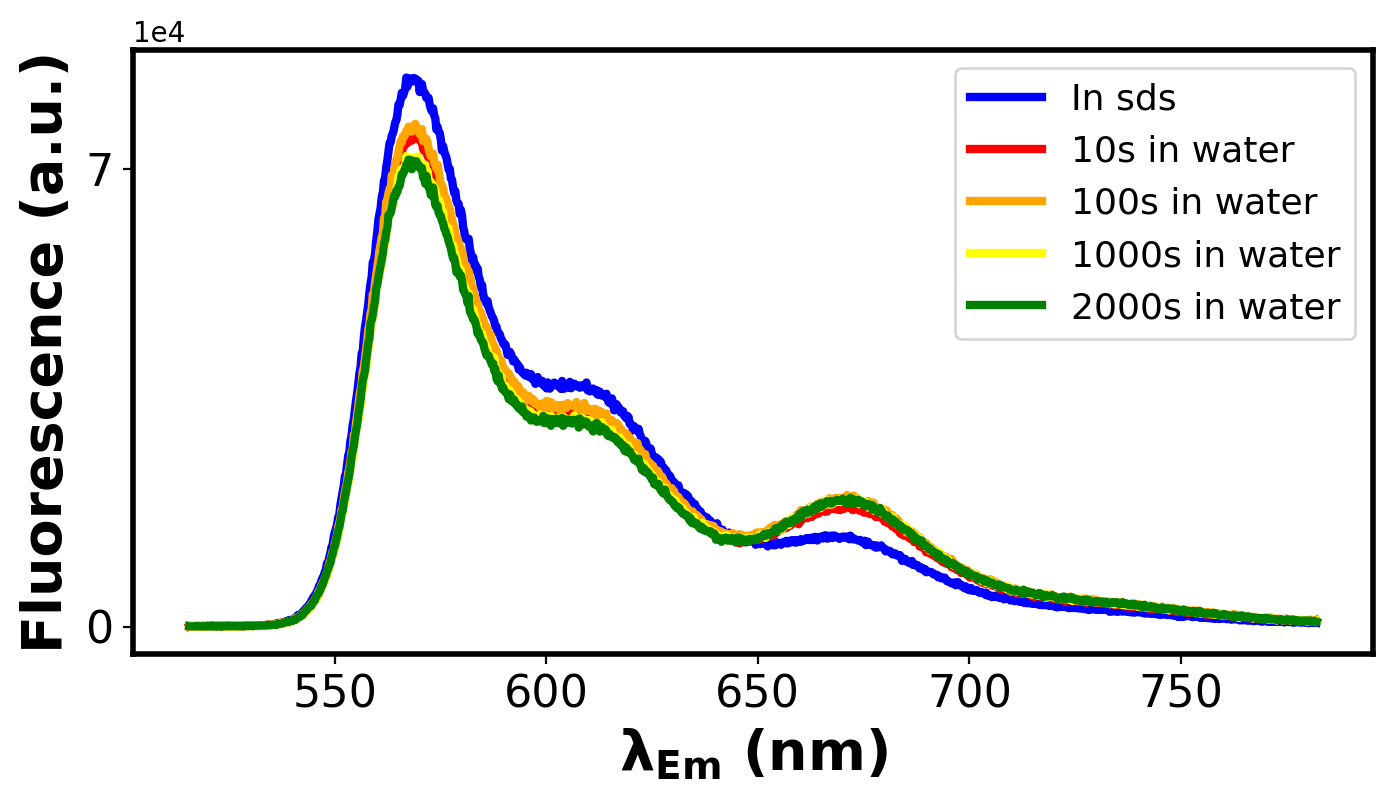
\includegraphics[width=\textwidth]{figures/chapter4/Fig4-6_watercontrol.png}
\end{center}
	\caption{\textbf{FRET measurements of KcsA tetramerization.} \textbf{(A)} Ensemble FRET measurement of the KcsA monomer in SDS and in liposome as a function of time \textbf{(B)} Double-jump (unfold-fold-unfold) FRET measurements of KcsA refolding quenched with 10\% SDS overlaid with ‘in sds’ and ‘10s in liposome time points’ from \textbf{(A)}. Spectra are normalized to have the same value at 641 nm, an empirical iso-emissive point. Measurements are conducted at a monomer concentration of 10 $\mu$M.}
	\label{fig:ch4_f7}
\end{figure}

\section{Conclusion}

Our investigation of the folding of potassium channel monomers and their role in assembly of potassium channel pores revealed a number of salient features. The MD simulations and MSM analysis indicate that for both Kv1.2 pore domain and KcsA, monomers form a heterogeneous ensemble of native and non-native states with all three helices folded and lying within the membrane. While the population of native-like states of the monomer is non-negligible (18\% for Kv1.2 and 44\% for KcsA), it is nevertheless striking that a considerable number of non-native states exists despite the substantial conformational restriction imposed by the environment; namely, the secondary structure of all three helices is retained, and the two TM helices remain inserted within the planes of the bilayer. Based on prior studies of hydrophobic matching36-39, the different lengths of TM helices presumably contribute to their tendency to separate.

This overall picture is consistent with our NMR data combined with prior thiol-labeling studies.20-21 Our attempts to generate well-resolved NMR spectra for the WT KcsA monomer inserted in nanodisc and bicelles were unsuccessful. Suspecting that the separation of the TM helices was the critical feature, a double cysteine variant was engineered to have a disulfide bond at the bottom of the two TM helices locking them into a native-like arrangement. This CC variant yielded a well-dispersed 1H-15N HSQC spectrum supporting the view that the WT’s TM helices were often separated in the monomers and formed a heterogeneous ensemble.

FRET-monitored refolding measurements of monomers passing from SDS into liposomes indicated that both WT $\Delta$125 and CC $\Delta$125 variants oligomerized well before the appearance of native tetramers. According to both SDS-resistance assays and FRET measurements, WT KcsA monomers assembled into native tetramers via two distinct kinetic paths with 40  2 and 1500  100 s. The CC variant largely if not fully lacked the slow phase. We posit that slow folding is the result of non-native packing arrangements of the TM helices that must ultimately be corrected for tetrameric assembly to proceed. The observation of slow and fast folding routes has been seen in many soluble proteins where the initial collapse step leads to species with native-like topology on a direct pathway, or to a species containing a partially misfolded structure that is slow to correct (Fig. 5).40-42

\begin{figure}[!ht]
\begin{center}
	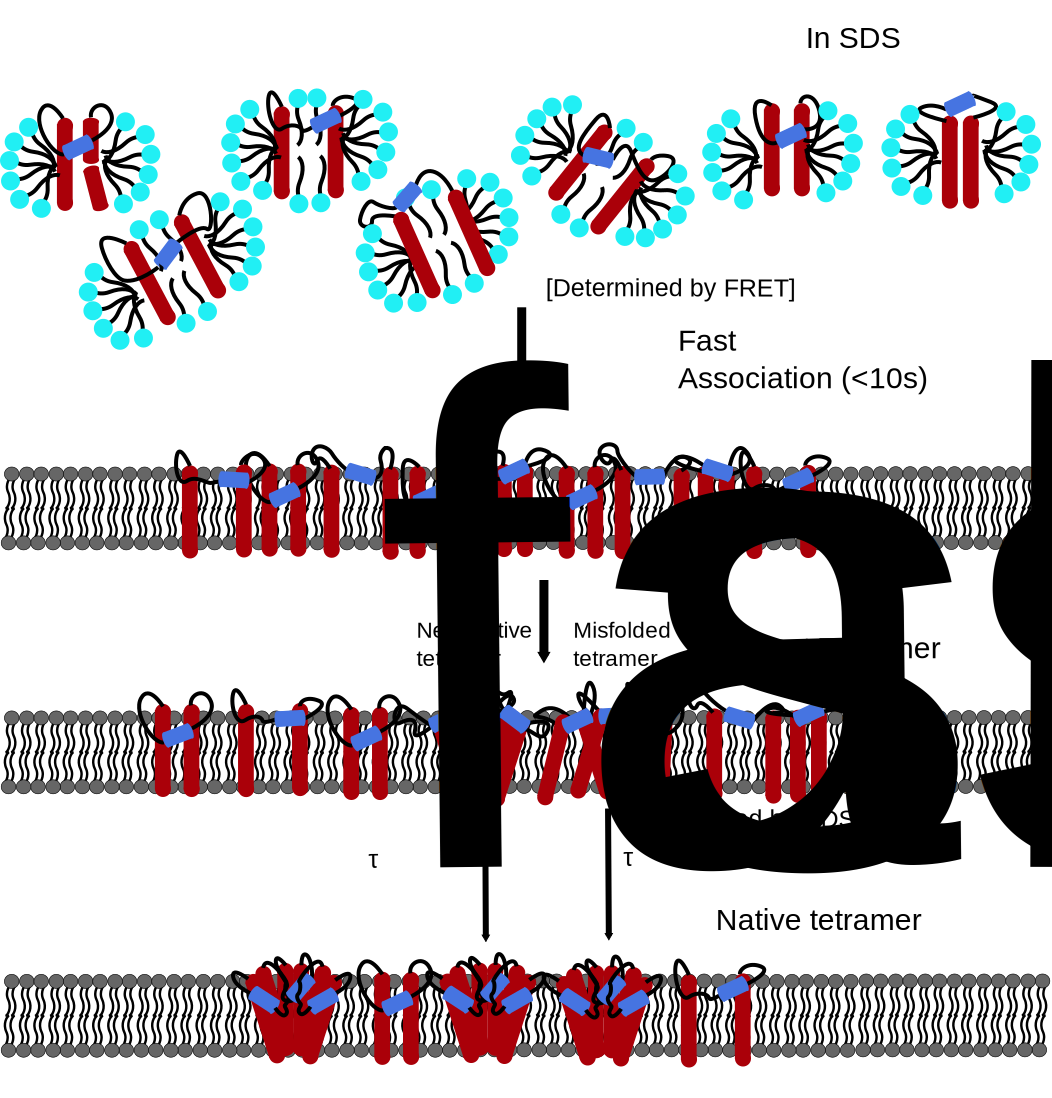
\includegraphics[width=\textwidth]{figures/chapter4/Fig4-7_summary.pdf}
\end{center}
	\caption{\textbf{Proposed KcsA folding and tetramerization.} SDS-solubilized monomers enter the liposomes and undergo rapid association into a protein-rich phase within the membrane prior to tetramerization. Oligomers can form with a native or non-native TM helical arrangement, which fold on the minute or 20 minute time scale, respectively, The rate limiting step on the faster pathway is proposed to involve the insertion of the pore helix to stabilize the tetramer in its native conformation.}
	\label{fig:ch4_f8}
\end{figure}

In spite of the channel being a tetramer, folding of the WT 125 and CC 125 constructs was concentration independent from 1 – 10 M for both the fast and slow phases, both in rate and amplitude. This observation implies that the rate-limiting step on both pathways is unimolecular. Because the FRET measurements indicated that the monomer insertion and oligomerization was relatively quick, the rate-limiting step on the fast pathway likely occurs going from an oligomer to a native tetramer. This complex transition requires the formation of the slightly twisted arrangement of the 8 TM helices, and the energetically costly opening of an aqueous channel. Final formation of native tetramers may occur in a concerted step with the association of correctly folded monomers already having the pore helices and selectivity filters positioned in a native or near-native orientation. Alternatively, this event may occur in two distinct steps, with the p-helices and selectivity filter segments folding into position only after the 8 TM have adopted their correct native arrangement. Further studies are needed to resolve this question.

The carboxy-terminal stalk domain in KcsA was tested to see if it enhanced tetramerization. In eukaryotic channels such as the Shaker voltage-activated potassium channel, the presence of the “tetramerization” T1 domain improves the rate of successful folding and assembly.13 Whereas the carboxy-terminal domain of KcsA forms a four-helix bundle that contributes to the stability of the folded tetrameric channel,43 its role in the assembly process is unclear. In other studies, the KcsA tetramerization domain alone has been shown to oligomerize in pH and concentration dependent manners44-45 as well as increase the stability of KcsA tetramers.33

However, the folding kinetics of KcsA pore domain with the tetramerization domain has not been extensively studied in the past. To our surprise, the presence of the tetramerization domain did not improve the channel’s folding behavior. For both the WT and CC variants, tetramerization became concentration dependent in a complex manner with both a reduced fast phase and lower overall yield of tetramers. One may consider that our refolding protocol with insertion into liposomes starting from an SDS-solubilized state does not properly mimic the biological context and so preclude the tetramerization domain for assisting folding. Also, the C-terminal region carries a net positive charge, which may cause a repulsion at large distance between monomers prior to tetramerization. Potentially the domain lends specificity and is more important for finding other KcsA subunits or improving the stability of tetramers once they are formed.

The folding of the potassium channels displays similar behavior to other -helical membrane proteins, having a transition state close to the native state.9-11 For example, in the force unfolding studies of GlpG pulling parallel to the bicelle surface, the transition state was closer to the native state than that observed in SDS-driven folding/unfolding studies in solution.46-47 In other SDS-based refolding studies on bacteriorhodopsin, DsbB and GlpG, the transition states were expanded.48-50 The observed difference between the force- and the SDS-driven unfolding studies may be due to the difference in the mode of denaturation as well as folding conditions (micelle or bicelle versus liposomes). Regardless, KcsA in liposomes appear to have a transition state near the native state.

The two-stage model, proposed nearly 30 years ago, has provided a useful framework for discussing membrane protein folding. The model, which posits insertion of all the TM helices followed by lateral packing, was proposed based on studies which observed that bacteriorhodopsin cut in a few pieces could still be re-assembled.51-53 With the observation of more diverse folding behaviors, a more sophisticated three-stage model10 was proposed where insertion and lateral packing of the TM helices could be followed by ligand binding, loop folding or peripheral domain insertion. This extra step is relevant to potassium channels, where the insertion of the four pore helices and the formation of the selectivity filter may be required to finalize the folding process.

For KcsA, the first two stages seem to correspond to insertion and formation of a protein-rich phase before folding into native tetrameric channels. This result brings up an interesting question in regards to membrane protein folding in general, namely, should the membrane be considered to be a good or poor solvent with respect to TM helices, defined as one where helix–lipid interactions are stronger or weaker, respectively, than helix–helix interactions. For potassium channels, a mixed behavior is observed. A protein-rich phase is detected by FRET, but the two TM helices in a monomer can dissociate from one other according to NMR (in bicelles) and MD simulations (POPC bilayers).

Potentially in the folding of other membrane proteins, non-specific or quinary interactions between TM helices also may give rise to a protein dense phase. These interactions can also occur in native structures, as seen with KcsA tetramers undergoing lateral association both in our and earlier studies.34-35 Several studies have shown that membrane proteins can alter lipid packing in the fluid liquid crystalline phase, which can in turn cause proteins to associate non-specifically in order to minimize the perturbation on the membrane.54-55 Generally, lipids may act as a marginally poor solvent for TM helices especially if the helices contain polar amino acids that are less soluble in the hydrophobic bilayer.56-62 These mixed results, along with variability of the hydrophobicity of the TM helices and the properties of the bilayer (e.g., composition, curvature, lateral pressure), suggest that solvent quality is likely system dependent. These issues have important implications to in vivo folding where helices partition between chamber of the translocon, lipid-water interface and the hydrophobic core of the membrane.63 

%% REVERT FIGURE NUMBERING %%
\renewcommand\thefigure{\thechapter.\arabic{figure}} 

%%% END CHAPTER 4 refolding studies %%%

